\subsection{Class diagram di analisi o dominio}

    \begin{flushleft}
        \begin{description}
            \item[Class diagram a livello concettuale] Studia i concetti propri del dominio sotto studio, senza preoccuparsi della loro successiva implementazione. È una sorta di Dizionario Visuale del dominio.
            \item[Class diagram di specifica implementativa] Rappresenta la struttura implementativa, specificando come va sviluppato il sistema. È un raffinamento del precedente.
          \end{description}

        I Class diagram di analisi o di dominio ci forniscono un'indicazione iniziale sulle componenti principali del software a prescindere 
        dall'architettura e dalle tecnlogie che verranno poi scelte per implementarli. 
        In questa fase infatti ancora di analisi, il team sta concretizzando i requisiti in qualcosa di pratico da dare in pasto ai programmatori, che 
        ne seguiranno il modello per arrivare al prodotto finito.

    \end{flushleft}

    \subsubsection{Class diagram Login}
        \begin{figure}[H]
            \centering
            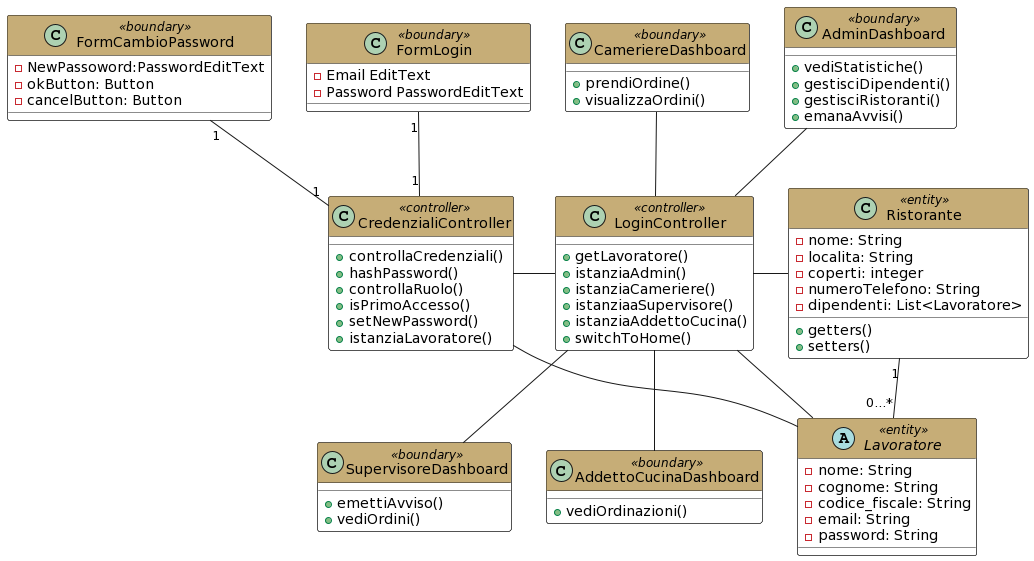
\includegraphics[scale=0.45]{assets/diagrammi/Class diagram di analisi/Gestione Login.png}
            \caption{\textbf{C01}: Class diagram Login}\label{fig:Login}
        \end{figure}

    \subsubsection{Class diagram Ristorante}
        \begin{figure}[H]
            \centering
            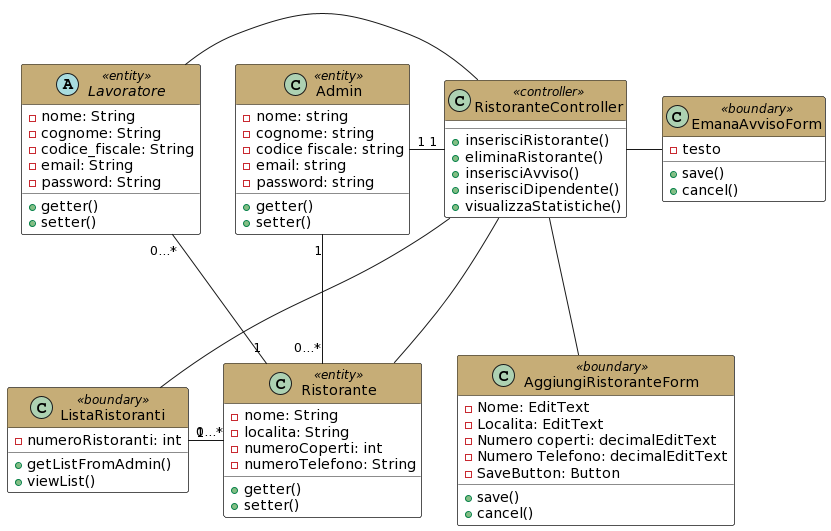
\includegraphics[scale=0.5]{assets/diagrammi/Class diagram di analisi/Gestione ristorante.png}
            \caption{\textbf{C02}: Class diagram Gestione ristorante}\label{fig:Ristorante}
        \end{figure}

    \subsubsection{Class diagram dipendenti}
        \begin{figure}[H]
            \centering
            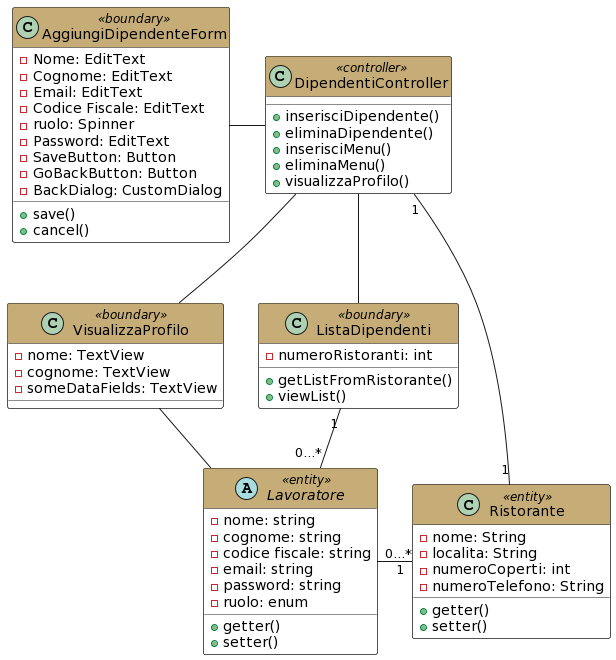
\includegraphics[scale=0.5]{assets/diagrammi/Class diagram di analisi/Gestione dipendenti.png}
            \caption{\textbf{C03}: Class diagram gestione dipendenti}\label{fig:Dipendenti}
        \end{figure}
    
    \subsubsection{Class diagram Menu}
        \begin{figure}[H]
            \centering
            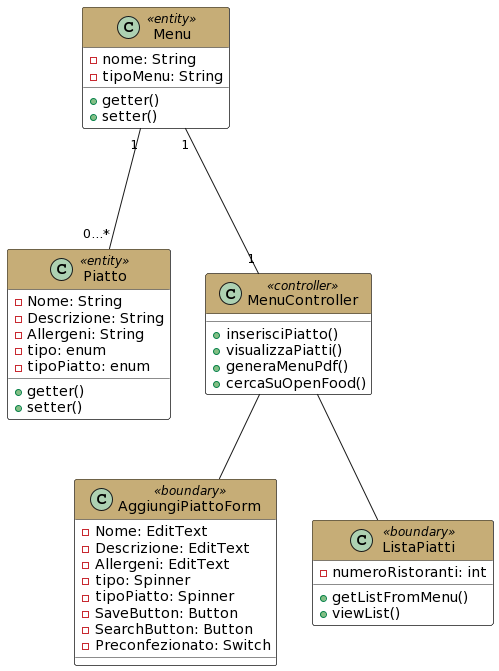
\includegraphics[scale=0.5]{assets/diagrammi/Class diagram di analisi/Gestione piatto.png}
            \caption{\textbf{C04}: Class diagram gestione piatti}\label{fig:Menu}
        \end{figure} 

    \subsubsection{Class diagram Avvisi}
        \begin{figure}[H]
            \centering
            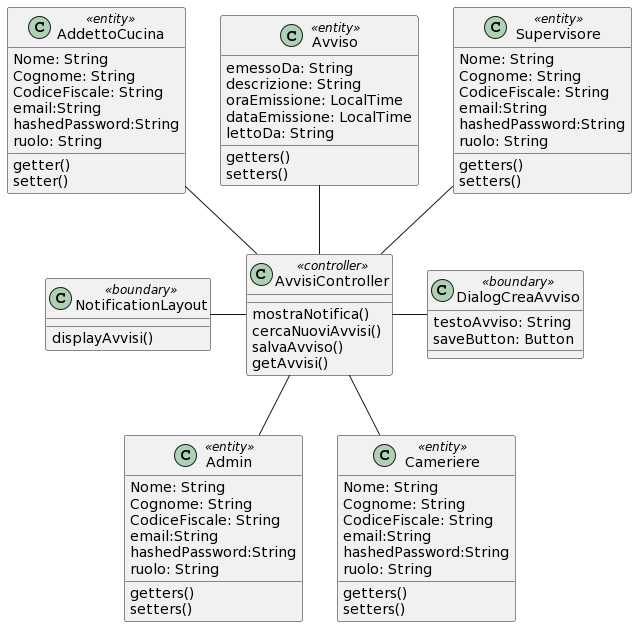
\includegraphics[scale=0.5]{assets/diagrammi/Class diagram di analisi/Gestione Avvisi.png}
            \caption{\textbf{C05}: Class diagram gestione avvisi}\label{fig:Avvisi}
        \end{figure}

    \subsubsection{Class diagram Ordini}
        \begin{figure}[H]
            \centering
            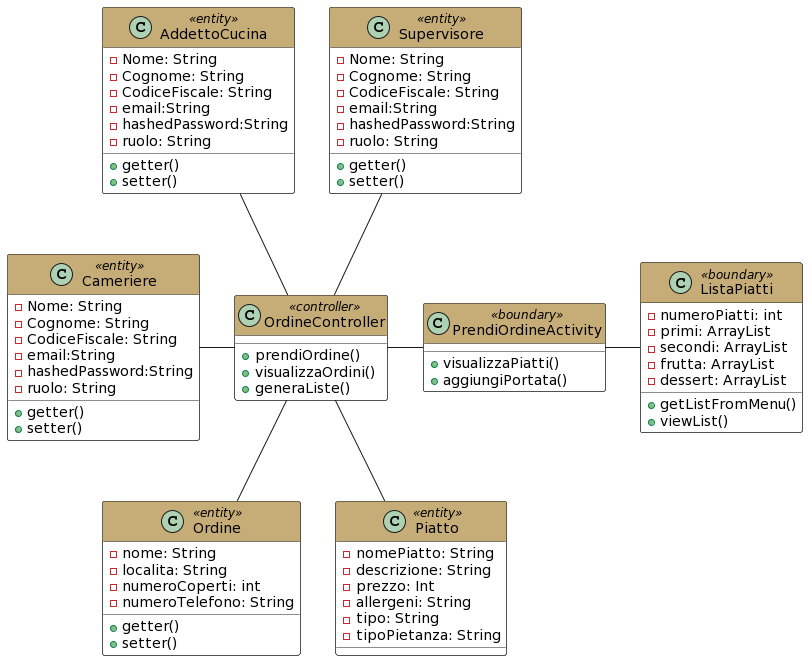
\includegraphics[scale=0.5]{assets/diagrammi/Class diagram di analisi/Gestione ordini.png}
            \caption{\textbf{C06}: Class diagram gestione ordini}\label{fig:Ordini}
        \end{figure}

    \subsubsection{Class diagram statistiche}
        \begin{figure}[H]
            \centering
            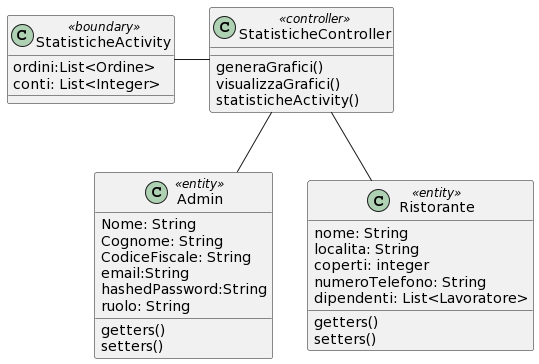
\includegraphics[scale=0.5]{assets/diagrammi/Class diagram di analisi/Gestione Stat.png}
            \caption{\textbf{C07}: Class diaram gestione statistiche}\label{fig:Statistiche}
        \end{figure}